% !Mode:: "TeX:UTF-8"
% !TEX program = xelatex
\section{概念澄清及初探}
概念的混淆容易引起不必要的争端,因此在讨论某一特定的问题时,应先澄清其中所有的概念,并与讨论者达成共识。所以在讨论题目“工具理性在现代社会的合理性”时,我首先需要明确什么是“工具理性”、“现代社会”。

首先,我需要定义“工具理性”。参考维基百科的 Instrumental and value rationality\cite{wiki2019instrumental_rationality},知道”工具理性“(Instrumentally Rational)是由 Max Weber 最先提出的,同时他也提出了另一种”价值理性“(Value-rational),而这一观点也不断由后人延伸解读着,比如 John Rawls,Robert Nozick 等。我规定,本文讨论的“工具理性”与”价值理性“均为 Weber 的原始定义:
\begin{enumerate}
    \item \textbf{Instrumentally rational (zweckrational)}, that is, determined by expectations as to the behavior of objects in the environment and of other human beings; these expectations are used as "conditions" or "means" for the attainment of the actor's own rationally pursued and calculated ends;
    \item \textbf{Value-rational (wertrational)}, that is, determined by a conscious belief in the value for its own sake of some ethical, aesthetic, religious, or other form of behavior, independently of its prospects of success.
\end{enumerate}
由定义可以看出,”工具理性“与”价值理性“之间不是对立,即”工具理性“是由〖环境中对象〗或〖人类行为〗的期望所决定的,而“价值理性”是由某种道德、审美、宗教或其他形式行为的价值所决定的,与成功无必然的关系。换言之:
\begin{quotation}
    价值理性相信的是一定行为的无条件的价值,强调的是\textbf{动机的纯正}和\textbf{选择正确的手段}去\textbf{实现自己意欲达到的目的},而\textbf{不管其结果如何}。而工具理性是指行动\textbf{只由追求功利的动机所驱使},行动\textbf{借助理性}达到自己需要的预期目的,行动者纯粹从\textbf{效果最大化的角度}考虑,而\textbf{漠视人的情感和精神价值}。\cite{mba2019工具理性}
\end{quotation}

同时,我对维基百科进行英文分词,并统计词频绘制词云如图~\ref{F:1}。出现最多的词汇除了”工具理性“与”价值理性“外,还有:
\begin{enumerate*}[label=(\alph*)]
    \item reasonable;
    \item moral;
    \item legitimate;
    \item utility;
    \item unconditionally;
    \item effective;
    \item conditional;
    \item paradox。
\end{enumerate*}
回查文章,与我目前理解的重点基本吻合。
\begin{figure}[H]
    \centering
    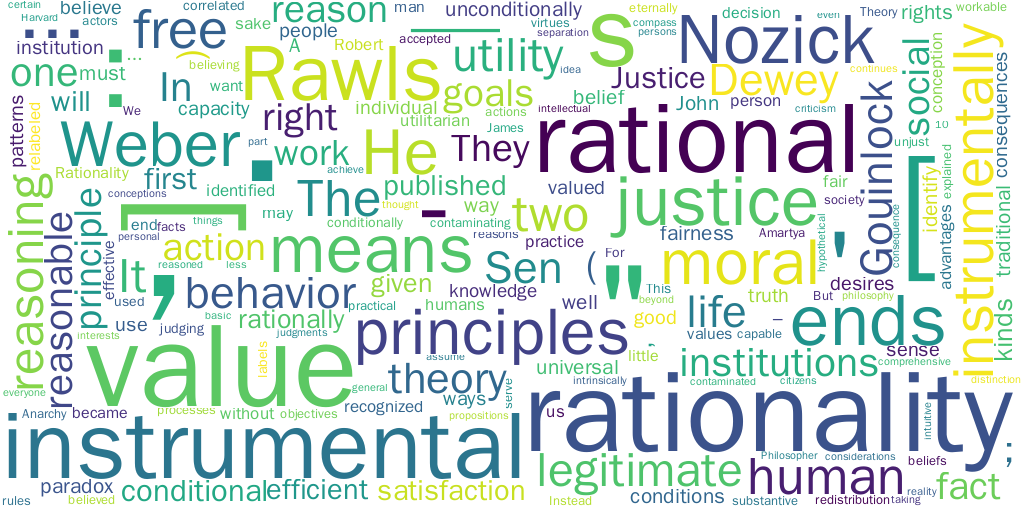
\includegraphics[width=.8\textwidth]{wordcloud/工具理性.png}
    \caption{“Instrumental and value rationality”词云}\label{F:1}
\end{figure}

接下来,我需要定义“现代社会”,参考知乎\cite{liu2017现代性}的回答,在阅读大量的回答论述中,我得到的始终是不确定的,即无法明确定义“现代社会”。因此对知乎的回答进行中文分词\cite{sun2019jieba},并统计词频绘制词云如图~\ref{F:2}。在剔除词频较高的词汇与停用词后,我得到许多无意义的词组(人名等),因此需要对高频词汇进行分析:
\begin{enumerate*}[label=(\alph*)]
    \item 理性;
    \item 生活;
    \item 领域;
    \item 冲突;
    \item 变革。
\end{enumerate*}
然而,高频词汇周围的句子同样无法定义“现代社会”,因此,此处按照作者的理解进行定义。如果将“现代社会”定义区间过长至启蒙运动则对现实缺乏了参考意义,所以在保证对现实存在参考价值的前提下,我们将本文章中的“现代社会”定义为自千禧年至今(一方面千禧年是重要的时间锚点,另一方面互联网在千禧年前后存在重大发展,参考摩尔定理)。
\begin{figure}[H]
    \centering
    
\includegraphics[width=.8\textwidth]{wordcloud/现代性.png}
    \caption{“知乎现代性回答”词云}\label{F:2}
\end{figure}

综上所述,通过技术手段的客观分析及阅读材料的主观判断,本文的题目可以进一步具体化,即“工具理性在互联网时代的合理性”,接下来,我将围绕这个题目进行分析。
